%%%%%%%%%%%%%%%%%%%%%%%%%%%%%%%%%%%%%%%%%%%%%%%%%%%%%%%%%%%%%%%%%%%%%%%%%%
%XX.XX - Nombre Materia
%Trabajo Prático XXX
%Tema
%%%%%%%%%%%%%%%%%%%%%%%%%%%%%%%%%%%%%%%%%%%%%%%%%%%%%%%%%%%%%%%%%%%%%%%%%%
%
% Tamaño de letra principal:
%

\documentclass[10pt]{article}
%
% Título y autor(es):
%
\title{JugaMe, Experimentando con Juegos}
\author{Simone Mariano}

%------------------------- Carga de paquetes ---------------------------
%
% Definición del tamaño de página y los márgenes:
%
\usepackage[a4paper,headheight=16pt,scale={0.7,0.8},hoffset=0.5cm]{geometry}

% Para escribir en castellano:
\usepackage[spanish]{babel}
\usepackage[utf8]{inputenc}

\usepackage{amsmath}
\numberwithin{equation}{section}
\numberwithin{figure}{section}
\numberwithin{table}{section}

% Para tener cabecera y pie de página con un estilo personalizado:
\usepackage{fancyhdr}

% Para poner el texto "Figura X" en negrita:
\usepackage[hang,bf]{caption}
\usepackage{multirow}
% Para poder usar subfiguras:
\usepackage{subfigure}

% Para poder agregar notas al pie en tablas:
\usepackage{threeparttable}



%------------------------------ graphicx ----------------------------------
%
% Para incluir imágenes, el siguiente código carga el paquete graphicx 
% segn se está generando un archivo dvi o un pdf (con pdflatex).
%
\newif\ifpdf
\ifx\pdfoutput\undefined
	\pdffalse
\else
	\pdfoutput=1
	\pdftrue
\fi

\ifpdf
	\usepackage[pdftex]{graphicx}
	\pdfcompresslevel=9
\else
	\usepackage[dvips]{graphicx}
\fi
% Para poder incluir graficos de dia directamente
\usepackage{tikz}
%
% Todas las imáenes está en el directorio tp-img:
%
\newcommand{\imgdir}{img}
\graphicspath{{\imgdir/}}
%
%------------------------------ graphicx ----------------------------------

%%%%%%%%%%%%%%%%%%%%%%%%%%%%%%%%%%%%%%%%%%%%%%%%%%%%%%%%%%%%%%%%%%%%%%%%%%%%%%%%
\usepackage{color}
\definecolor{gray75}{gray}{.75}

\definecolor{listinggray}{gray}{0.9}
\definecolor{lbcolor}{rgb}{0.9,0.9,0.9}

\usepackage{listings}
\usepackage{textcomp}
\lstset{
	backgroundcolor=\color{lbcolor},
	tabsize=4,
	rulecolor=,
	language=C++,
        basicstyle=\scriptsize,
        upquote=true,
        aboveskip={1.5\baselineskip},
        columns=fixed,
        showstringspaces=false,
        extendedchars=true,
        breaklines=true,
        prebreak = \raisebox{0ex}[0ex][0ex]{\ensuremath{\hookleftarrow}},
        frame=single,
        showtabs=false,
        showspaces=false,
        showstringspaces=false,
        identifierstyle=\ttfamily,
        keywordstyle=\color[rgb]{0,0,1},
        commentstyle=\color[rgb]{0.133,0.545,0.133},
        stringstyle=\color[rgb]{0.627,0.126,0.941},
}
%Ejemplo de uso para incluir un archivo: \lstinputlisting{parameters.py}
%Ejemplo para codigo inline: \begin{lstlisting} \end{lstlisting}

%%%%%%%%%%%%%%%%%%%%%%%%%%%%%%%%%%%%%%%%%%%%%%%%%%%%%%%%%%%%%%%%%%%%%%%%%%%%%%%%
\usepackage{hyperref}
\hypersetup{
            pdftitle=JugaMe - Experimentando con Juegos,%
            pdfauthor=Mariano Simone,%
            pdfsubject=Desarrollo de DSL para Teoría de Juegos,%
            pdfkeywords=dsl ruby juegos,%
            colorlinks,%
            citecolor=black,%
            filecolor=black,%
            linkcolor=black,%
            urlcolor=black,%
            pdftex}


%------------------------- Inicio del documento ---------------------------

\begin{document}

%Así el caption de las tablas dice Tabla, y no Cuadro
\renewcommand{\tablename}{Tabla}

%
% Hago que en la cabecera de página se muestre a la derecha la sección,
% y en el pie, en nmero de página a la derecha:
%
\pagestyle{fancy}
\renewcommand{\sectionmark}[1]{\markboth{}{\thesection\ \ #1}}
\lhead{}
\chead{}
\rhead{\rightmark}
\lfoot{}
\cfoot{}
\rfoot{\thepage}

%
% Caráula:
%
\begin{titlepage}
%
% Sin cabecera ni pie de página:
%
	\thispagestyle{empty}
%
% Logo de la facu arriba a la izquierda: 
%
	
\includegraphics[scale=0.7]{logo-facu}
	\vfill
%
% Título:
%
	\begin{center}
		\Huge{Jugame}\\
		\vspace{1cm}
		\LARGE{Experimentando con Juegos}\\
		\vspace{1cm}
		
\includegraphics[scale=0.5]{logo-jugame}
	\end{center}
	\vspace{2cm}
%
% Integrantes:
%
	\large{
			Simone, Mariano Sebastián\\
			Padrón: 85609\\		
	}
	\vfill
%
% Fecha o cuatrimestre:
%
\end{titlepage}

%
% Hago que las páginas se comiencen a contar a partir de aquí
%
\setcounter{page}{1}

%
% Pongo el índice en una página aparte:
%
\tableofcontents
\newpage


\section{Objetivo}
En el presente trabajo se persiguen, principalmente, dos objetivos.
Por un lado, en cuanto al objeto de estudio, se busca investigar y desarrollar sobre el paradigma de Domain Specific Languages (DSLs), en el contexto de Object Oriented Programming (OOP).
Por otro lado, en lo referente a la aplicación práctica, se intenta profundizar en los conocimientos previamente adquiridos en la simulación y apoyo en la toma de decisiones en las situaciones típicas estudiadas por la Teoría de Juegos.

\section{Metas}\label{metas}
\begin{list}{*}{}
  \item Analizar la implementación de algún DSL para observar mejores prácticas y potenciales problemas, en particular, Rake
  \item Desarrollar un DSL que permita
  \begin{list}{-}{}
    \item Definir situaciones de juego (alternativas de acción y matriz de pagos asociada)
    \item Definir estrategias de juego
    \item Simular el desarrollo de partidas de las estrategias en los juegos definidos
  \end{list}
  \item Utilizar la metodología Behaviour Driven Development\footnote{http://behaviour-driven.org/} en el desarrollo (a través de RSpec\footnote{http://rspec.info/})
\end{list}

\section{Motivación}\label{motivacions}
Habiendo adquirido conocimientos básicos sobre Teoría de Juegos en materias dictadas en la Facultad de Ingeniería\footnote{Análisis y Resolución de Problemas de Sistemas y Modelos y Optimización III}, y tras leer la obra de los mayores referentes del área\cite{Axe:01}\cite{Axe:02} (con particular interés en ``Evolving New Strategies'', de Robert Axelrod), se elegió este tema como centro de un trabajo grupal. En el mismo, se hizo hincapié en la resolución de un juego particular (inventado especialmente para la ocasión), mediante diversas estrategias automáticas, haciéndolas competir para poder establecer un orden relativo de capacidad de juego entre ellas (con el fin último de hacerlas competir contra jugadores humanos). Durante el desarrollo, surgieron claros indicios de que era posible agrupar gran parte del comportamiento común de las estrategias, y modificar pequeñas porciones, logrando comportamientos totalmente distintos. De la misma manera, se hizo evidente que la estructura de la mayor parte de las situaciones estudiadas por dicha disciplina era similar. Con todo esto, me surgió el interés por desarrollar una biblioteca que permita la definición de juegos y estrategias de manera sencilla y directa.\\

Por otro lado, el creciente interés, por parte de la comunidad de desarrollo de Software en general, y por grandes referentes en particular (como el caso de Martin Fowler\cite{Fow:01}), por los Lenguajes Específicos de un Dominio\footnote{Es creciente el número de artículos relacionados con DSLs en sitios como InfoQ: http://www.google.com/search?q=dsl+site\%3Awww.infoq.com}, generó la curiosidad suficiente como para elegirlo como paradigma en el cual implementar la solución.

\newpage
\section{Teoría de Juegos}\label{juegos}
La Teoría de Juegos es el área de la matemática aplicada que utiliza modelos para estudiar interacciones en estructuras formalizadas de incentivos y llevar a cabo procesos de decisión. Estudia las estrategias óptimas, así como el comportamiento previsto y observado de los individuos.\\

Desarrollada en sus comienzos como una herramienta para entender el comportamiento de la economía, la Teoría de Juegos se usa actualmente en una amplia gama de disciplinas, desde la biología a la filosofía. Experimentó un crecimiento sustancial y se formalizó por primera vez a partir de los trabajos de John von Neumann y Oskar Morgenstern, antes y durante la Guerra Fría, debido sobre todo a su aplicación a la estrategia militar. Desde los setenta y hasta la actualidad, también se la ha ido aplicado a la conducta animal, la  economia, ciencias políticas, ética y filosofía, en la inteligencia artificial y cibernética.\\

Aunque tiene algunos puntos en común con la Teoría de la Decisión, la Teoría de Juegos estudia decisiones realizadas en entornos donde las mismas interaccionan. En otras palabras, estudia la elección de la conducta óptima cuando los costes y los beneficios de cada opción no están fijados de antemano, sino que dependen de las elecciones de otros individuos.\\

Los analistas utilizan asiduamente otras áreas de la matemática, en particular las probabilidades, las estadísticas y la programación lineal, en conjunto con la Teoría de Juegos.\cite{Wiki:01}

\subsection{Situaciones de Juego}
Los juegos estudiados por esta disciplina se definen mediante objetos matemáticos. Un juego consiste en:

\begin{list}{*}{}
  \item Un conjunto de jugadores
  \item Un conjunto de movimientos disponible para esos jugadores
  \item Una especificación de recompensas para cada combinación de movimientos elegidos (llamada Matriz de Pagos)
\end{list}

Dados esos tres conjuntos, el desarrollo del juego se entiende como la elección de cada jugador de uno de los movimientos posibles, y el otorgamiento de puntos (o pagos) a cada uno de ellos, según la especificación.\\

Un juego típico y ampliamente conocido que puede ser estudiado por la Teoría de Juegos es ``Piedra, Papel o Tijera'', en donde:

\begin{list}{*}{}
  \item Los jugadores son dos
  \item Los movimientos posibles son Piedra, Papel y Tijera
  \item La Matriz de Pagos es como sigue
\end{list}

\begin{table}[h]
\begin{center}
  \begin{tabular}{|c|c|c|c|}
  \hline
  & Piedra & Papel & Tijera \\
  \hline
  Piedra & 0,0 & 0,1 & 1,0 \\ \hline
  Papel & 1,0 & 0,0 & 0,1 \\ \hline
  Tijera & 0,1 & 1,0 & 0,0 \\ \hline
  \end{tabular}
  \caption{Matriz de Pagos de ``Piedra, Papel o Tijera''}
  \end{center}
\end{table}

Situaciones menos lúdicas pueden ser tratadas de la misma manera (de ahí la relevancia de esta disciplina), generando un marco formal preestablecido con el cual analizar de manera objetiva un conflicto y apoyar la toma de decisiones.

\subsubsection{Casos particulares: Votación}
Siguiendo el esquema básico de una matriz de pagos, generada a partir de ciertas decisiones, se estudian casos especiales de construcción de la misma, aumentando la cantidad de situaciones diferentes en las que se pueden utilizar los métodos de análisis de Teoría de Juegos.\\

Un caso especial, es el de votación. En el mismo, cierta cantidad de jugadores tienen cierta preferencia sobre determinado aspecto (el objeto de la votación). Cada uno, obtendrá una ganancia proporcional a su preferencia sobre el elemento que haya salido ganador. Existen, además, reglas sobre cómo se contabilizarán los votos (cuánto vale cada voto y forma de desempatar).\\

Un ejemplo trivial de este caso es el siguiente:\\

Un grupo familar compuesto por el Padre, la Madre y la Hija deben decidir a qué lugar irán de vacaciones este verano. Las opciones son Villa General Belgrano (Córdoba), Pinamar (Buenos Aires) y Viedma (Río Negro). Dadas las afinidades de cada uno, el Padre prefiere ir al pueblo Cordobés (gusta de la cerveza y las comidas alemanas), la Hija a la costa bonaerense (sus amigas irán allí con sus familias) y la Madre, a la capital patagónica (tienen familiares viviendo ahí). Como cabe la posibilidad de empate, en caso de suceder gana el voto de la madre. A su vez, cada uno tiene una segunda y una tercera preferencia (la segunda opción del padre es Viedma, de la madre Pinamar y de la hija, Gral. Belgrano). Suponiendo que los tres quieren viajar, y que prefieren ir a cualquier lado antes que no hacerlo, se puede formalizar la situación de la siguiente manera:\\

\begin{list}{*}{}
  \item Los jugadores son Padre, Madre e Hija
  \item Los movimientos posibles son votar por Villa General Belgrano, por Pinamar o por Viedma
  \item La Matriz de Pagos es como sigue
\end{list}

\begin{table}[!ht]
\begin{center}
  \begin{tabular}{|c|c|c|c|c|c|}
  \hline
  
 \multicolumn{3}{|c|}{\multirow{2}{*}{}} & \multicolumn{3}{|c|}{Madre} \\ \cline{4-6}
 \multicolumn{3}{|c|}{} & Gral. Belgrano & Pinamar & Viedma \\ \hline
 \multirow{3}{*}{Padre = Gral. Belgrano}
 & \multirow{3}{*}{Hija}
   & Gral. Belgrano & 3,2,1 & 3,2,1 & 3,2,1\\ \cline{3-6}
   & & Pinamar & 3,2,1 & 1,3,2 & 2,1,3 \\ \cline{3-6}
   & & Viedma & 3,2,1 &2,1,3 & 2,1,3 \\ \hline
   \multirow{3}{*}{Padre = Pinamar}
 & \multirow{3}{*}{Hija}
   & Gral. Belgrano & 3,2,1 & 1,3,2 & 2,1,3\\ \cline{3-6}
   & & Pinamar & 1,3,2 & 1,3,2 & 1,3,2 \\ \cline{3-6}
   & & Viedma & 2,1,3 & 1,3,2 & 2,1,3 \\ \hline
   \multirow{3}{*}{Padre = Viedma}
 & \multirow{3}{*}{Hija}
   & Gral. Belgrano & 3,2,1 & 2,1,3 & 2,1,3\\ \cline{3-6}
   & & Pinamar & 2,1,3 & 1,3,2 & 2,1,3 \\ \cline{3-6}
   & & Viedma & 2,1,3 & 2,1,3 & 2,1,3 \\ \hline
  \end{tabular}
  \caption{Matriz de Pagos de ``Vacaciones en Familia''}
  \end{center}
\end{table}

\subsection{Necesidad de uso de herramientas automatizadas}
Como puede verse, a medida que se incrementan la cantidad de jugadores y la cantidad de opciones, la complejidad del problema crece exponencialmente, por lo que es muy útil el uso de computadoras para realizar el análisis necesario para elegir la estrategia más conveniente, así como calcular los resultados esperados al utilizar cada una de ellas.\\

En conjunto con técnicas de simulación, es relativamente sencillo generar entornos en los cuales observar los resultados posibles ante diferentes estrategias utilizadas, sin incurrir en los costos ni en los riesgos de tener que probar en situaciones reales. 
\begin{figure}[!ht]
\centering
\mbox{\subfigure{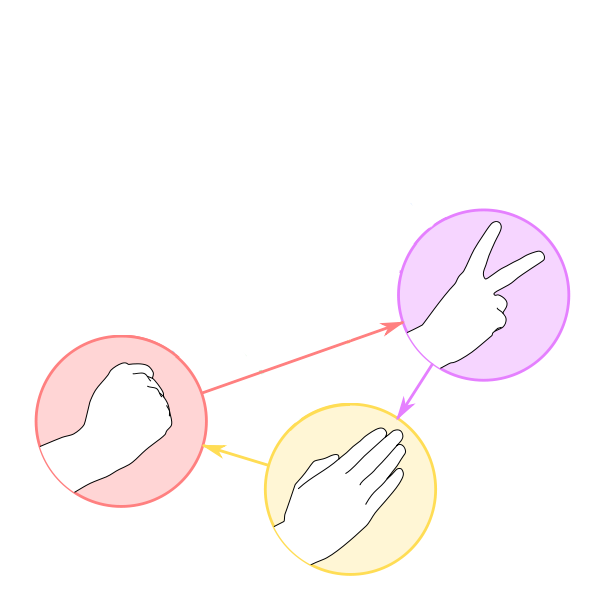
\includegraphics[width=3in]{rsp.png}}\quad
\subfigure{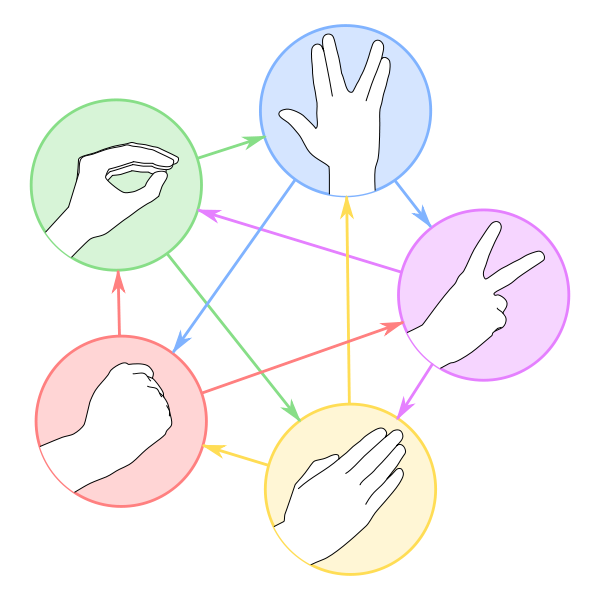
\includegraphics[width=3in]{rspls.png} }}
\caption{El aumento lineal de opciones genera aumento exponencial de complejidad} 
\end{figure}


\subsection{Análisis de juegos reitreados}
A fin de poder calcular estádisticas sobre los resultados obtenidos mediante una determinada estrategia (entendiendo a la misma como un algoritmo que decide qué decisión tomar en una situación de juego), se debe jugar una cierta cantidad de veces, así como comprobar la performance de la misma ante otras. Robert Axelrod\footnote{http://www-personal.umich.edu/~axe} es uno de los pioneros en el estudio del comportamiento de estrategias en juegos reiterados, habiendo propuesto un torneo entre diferentes algoritmos que decidan en el ``Dilema del Prisionero''\footnote{Uno de los juegos más simples y conocidos estudiados por la Teoría de Juegos, puede verse su definición en http://es.wikipedia.org/wiki/Dilema\_del\_prisionero} y establecido la forma de compararlas. El método elegido fue hacer que cada una de las estrategias propuestas compitiera contra cada una de las mismas, en rondas de cierta cantidad de jugadas, y analizar el puntaje acumulado obtenido por cada una.\cite{Axe:01}\\

Análisis de este estilo permiten obtener ciertas reglas que son comunes a las estrategias más exitosas y a las que menos victorias alcanzan. Cabe destacar que, cualquier estrategia que no logre superar a una aleatoria, automáticamente es descartada, ya que equivaldría a una decisión tomada sin tener en consideración ningún aspecto.

\newpage

\section{Domain Specific Languages}\label{dsls}
Un DSL en un lenguaje o especificación de programación o modelado, dedicado especialmente a un dominio de negocio particular. Dada la amplitud de esta definición, no existe un concenso en cuanto a qué puede ser considerado un DSL y qué no, aunque existen ciertos casos para los que no hay discusión:\\

No se consideran, por ser lenguajes de propósito general, DSLs:
\begin{list}{*}{}
  \item C, C++, Java, C\#
  \item Python, Ruby
  \item UML (sobre todo las versiones más modernas)
  \item PHP
\end{list}

Por otro lado, se consideran DSLs:
\begin{list}{*}{}
  \item  \TeX{}
  \item SQL
  \item CSS
  \item Expresiones Regulares
  \item SVG
\end{list}

Tomando como referente a Martin Fowler, también puede considera un DSL a todo aquel lenguaje que permita tratar a las entidades intervinientes (Clases, en el caso de OOP) como entidades directas del dominio. Por ejemplo, en Capistrano\footnote{Herramienta que permite automatizar tareas en servidores remotos (por ejemplo, todas las necesarias para deployar una aplicación): http://www.capify.org}, se trata a las entidades Tarea como tareas en sí, permitiendo definirle descripciones, precondiciones, su función, post-funciones, etc., sin hacer pensar al usuario en las particularidades de la OOP (como Herencia o Polimorfismo). Una crítica común a esta definición es que no se trata de más que \textit{Syntactic sugar}, y que un verdadero DSL debe prescindir de las abstracciones que no son de dominio (por ejemplo, en SQL una Tabla \textbf{es} una Tabla, y no una Clase que \textbf{representa} una Tabla)\\

Para, de alguna manera, escapar a esta crítica, el autor diferencia entre DSLs Internos y Externos\cite{Fow:01}. En el primer caso, se trata de usar un lenguaje \textit{host} (cuanto más flexible sea éste en su sintaxis y semántica, más sencilla será la implementación) de una manera distinta a la habitual, con el fin de crear un leguaje que se acerque lo más posible al dominio elegido. Por otro lado, los DSLs externos poseen su propia sintaxis y se debe desarrollar un parser para procesarlos. En este caso, cuanto mayor sea la flexibilidad deseada, tanto más compleja tendrá que ser la implementación.\\

Sin embargo, el mismo autor entiende que, desde el punto de vista práctico, suele ser muy útil concentrarse en el modelo en sí, ya que será éste el que de soporte a las capacidades del DSL, y luego probar generar varios DSLs internos que se encarguen de popular y configurar ese modelo, a fin de obtener el resultado deseado.\cite{Fow:03}\\

Un error común es confundir la cercanía del lenguaje en cuestión y el lenguaje de dominio con la cercanía al lenguaje natural. Si bien es una adición valiosa y que puede ayudar en el proceso de adopción del mismo, se debe tener en cuenta que el objetivo principal es acercarse a la expresividad necesaria por el dominio y no necesariamente a la humana. En otras palabras, se debe preponderar la creación de abstracciones del dominio por sobre las construcciones sintácticas de un lenguaje natural.

\newpage
\subsection{Implementación}\label{implementacion}
\subsubsection{Lenguage y Bibliotecas}
Se optó por diseñar e implementar un DSL Interno dado que, al evitar la implementación de las herramientas necesarias para un DSL externo (analizador, parser, compilador, etc.), se puede mantener una visión de alto nivel completa en un período relativamente corto de tiempo.\\

El lenguaje elegido para la implementación del DSL es Ruby\footnote{http://www.ruby-lang.org}, dada la flexibilidad de su sintaxis, la versatilidad y completitud de su biblioteca standard, así como el conocimiento previo del mismo. Además, la posibilidad de añadir métodos y definir clases dinámicamente, fué un factor decisivo a la hora de hacer la elección, ya que esto permite generar una nueva sintaxis muy clara, limpia y cercana al lenguaje del dominio.\\

En cuanto a las bibliotecas utilizadas, sólo fue necesario incorporar RSpec, como framework para realizar las pruebas que condujeron el desarrollo, pero cabe destacar que se podría reemplazar por cualquier otro, sin afectar en lo más mínimo al DSL.

\subsubsection{Esquema de la solución}
\begin{figure}[!ht]
\centering
    % Graphic for TeX using PGF
% Title: /home/mariano/Dropbox/fiuba/7539/jugame/doc/src/esquema.dia
% Creator: Dia v0.97
% CreationDate: Tue Mar  2 18:25:49 2010
% For: mariano
% \usepackage{tikz}
% The following commands are not supported in PSTricks at present
% We define them conditionally, so when they are implemented,
% this pgf file will use them.
\ifx\du\undefined
  \newlength{\du}
\fi
\setlength{\du}{15\unitlength}
\begin{tikzpicture}
\pgftransformxscale{1.000000}
\pgftransformyscale{-1.000000}
\definecolor{dialinecolor}{rgb}{0.000000, 0.000000, 0.000000}
\pgfsetstrokecolor{dialinecolor}
\definecolor{dialinecolor}{rgb}{1.000000, 1.000000, 1.000000}
\pgfsetfillcolor{dialinecolor}
\definecolor{dialinecolor}{rgb}{1.000000, 1.000000, 1.000000}
\pgfsetfillcolor{dialinecolor}
\pgfpathellipse{\pgfpoint{16.719266\du}{11.549996\du}}{\pgfpoint{8.499996\du}{0\du}}{\pgfpoint{0\du}{8.499996\du}}
\pgfusepath{fill}
\pgfsetlinewidth{0.100000\du}
\pgfsetdash{}{0pt}
\pgfsetdash{}{0pt}
\definecolor{dialinecolor}{rgb}{0.000000, 0.000000, 0.000000}
\pgfsetstrokecolor{dialinecolor}
\pgfpathellipse{\pgfpoint{16.719266\du}{11.549996\du}}{\pgfpoint{8.499996\du}{0\du}}{\pgfpoint{0\du}{8.499996\du}}
\pgfusepath{stroke}
\definecolor{dialinecolor}{rgb}{1.000000, 1.000000, 1.000000}
\pgfsetfillcolor{dialinecolor}
\pgfpathellipse{\pgfpoint{16.719300\du}{11.550000\du}}{\pgfpoint{5.000000\du}{0\du}}{\pgfpoint{0\du}{5.000000\du}}
\pgfusepath{fill}
\pgfsetlinewidth{0.100000\du}
\pgfsetdash{}{0pt}
\pgfsetdash{}{0pt}
\definecolor{dialinecolor}{rgb}{0.000000, 0.000000, 0.000000}
\pgfsetstrokecolor{dialinecolor}
\pgfpathellipse{\pgfpoint{16.719300\du}{11.550000\du}}{\pgfpoint{5.000000\du}{0\du}}{\pgfpoint{0\du}{5.000000\du}}
\pgfusepath{stroke}
% setfont left to latex
\definecolor{dialinecolor}{rgb}{0.000000, 0.000000, 0.000000}
\pgfsetstrokecolor{dialinecolor}
\node[anchor=west] at (15.372100\du,11.850000\du){Modelo};
% setfont left to latex
\definecolor{dialinecolor}{rgb}{0.000000, 0.000000, 0.000000}
\pgfsetstrokecolor{dialinecolor}
\node[anchor=west] at (15.441000\du,5.327500\du){Azúcar};
% setfont left to latex
\definecolor{dialinecolor}{rgb}{0.000000, 0.000000, 0.000000}
\pgfsetstrokecolor{dialinecolor}
\node[anchor=west] at (25.900000\du,7.027500\du){API};
% setfont left to latex
\definecolor{dialinecolor}{rgb}{0.000000, 0.000000, 0.000000}
\pgfsetstrokecolor{dialinecolor}
\node[anchor=west] at (25.900000\du,4.417500\du){DSL};
% setfont left to latex
\definecolor{dialinecolor}{rgb}{0.000000, 0.000000, 0.000000}
\pgfsetstrokecolor{dialinecolor}
\node[anchor=west] at (28.850000\du,4.950000\du){};
\pgfsetlinewidth{0.100000\du}
\pgfsetdash{}{0pt}
\pgfsetdash{}{0pt}
\pgfsetbuttcap
{
\definecolor{dialinecolor}{rgb}{0.490196, 0.474510, 0.474510}
\pgfsetfillcolor{dialinecolor}
% was here!!!
\pgfsetarrowsend{stealth}
\definecolor{dialinecolor}{rgb}{0.490196, 0.474510, 0.474510}
\pgfsetstrokecolor{dialinecolor}
\draw (23.327494\du,6.124668\du)--(25.550000\du,4.300000\du);
}
\pgfsetlinewidth{0.100000\du}
\pgfsetdash{}{0pt}
\pgfsetdash{}{0pt}
\pgfsetbuttcap
{
\definecolor{dialinecolor}{rgb}{0.490196, 0.474510, 0.474510}
\pgfsetfillcolor{dialinecolor}
% was here!!!
\pgfsetarrowsend{stealth}
\definecolor{dialinecolor}{rgb}{0.490196, 0.474510, 0.474510}
\pgfsetstrokecolor{dialinecolor}
\draw (21.206147\du,9.237378\du)--(25.450000\du,7.050000\du);
}
\end{tikzpicture}

\caption{Encapsulamiento progresivo del modelo}
\end{figure}

Utilizando la metodología Behaviour Driven Development, se generaron, progresivamente, las tres partes que constituyen la solución final.\\

Por un lado, se extendió la biblioteca standard de Ruby mediante la reapertura de ciertas clases (en particular: Array y Range) y la creación de otras (LovelyParent, aunque, en realidad, sea un Módulo y no una Clase) a fin de proveer métodos utilitarios que simplifiquen la sintaxis general.\\

Por otro lado, se implementaron las clases que modelan las entidades propias del dominio, como son Juego, Estrategia y Matriz de Pagos.\\

Finalmente, se desarrolló un DSL capaz de utilizar la API provista por el modelo para generar, popular, configurar y utilizar instancias de las entidades del mismo.

\subsubsection{Modelo}
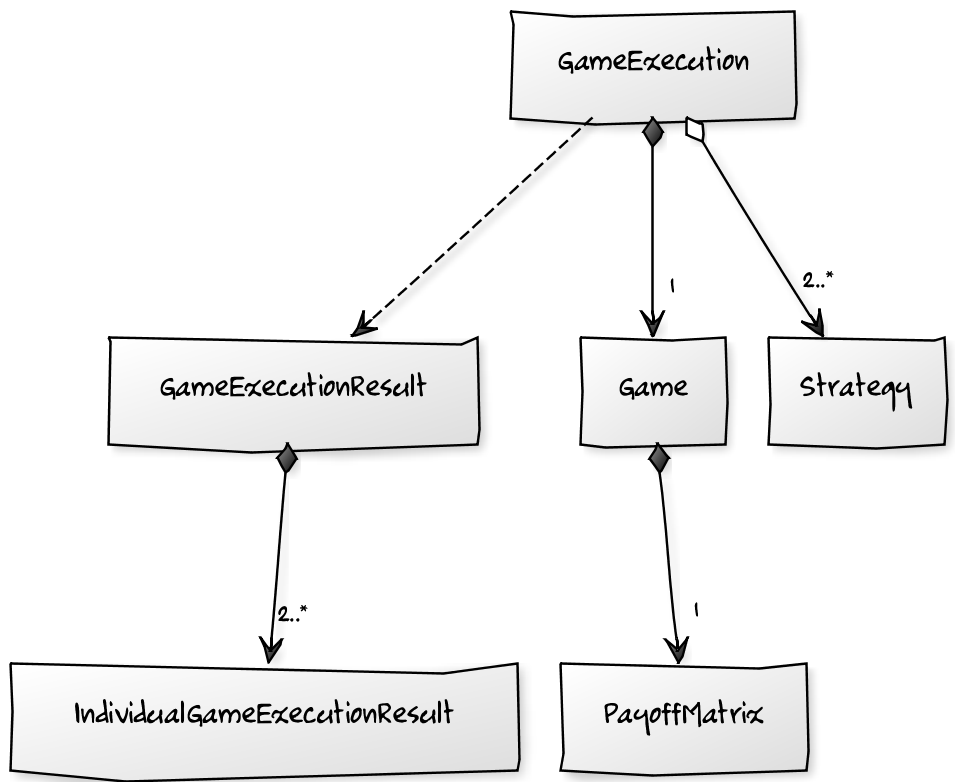
\includegraphics[width=15cm]{model.png}
Siendo el ilustrado el esquema del modelo implementado, se puede ver a continuación un ejemplo de su uso para la definición del Dilema del Prisionero:
\begin{lstlisting}
    game = JugaMe::Game.new("The Prissioner's Dilemma",2)
    game.add_moves(["Stay Silent", "Betray"])
    game.set_payoff ["Stay Silent", "Stay Silent"], [1, 1]
    game.set_payoff ["Stay Silent", "Betray"], [10, 0]
    game.set_payoff ["Betray", "Stay Silent"], [0, 10]
    game.set_payoff ["Betray", "Betray"], [5, 5]
\end{lstlisting}
En el mismo contexto, se puede ver la utlización de la misma definción, dentro de una ejecución:
\begin{lstlisting}
    execution = GameExecution.new(game, [JugaMe::RandomStrategy.new(game.moves),JugaMe::RandomStrategy.new(game.moves)])
    execution.play(10)
    results = execution.individual_results
\end{lstlisting}

\subsubsection{DSL}
Mediante la construcción de métodos estáticos que funcionan como builders y la apertura de la clase Object (raíz de toda la jerarquía de clases en Ruby), se construyó el DSL, permitiendo reescribir el código anterior como:\\

\begin{lstlisting}
    in_the_game "The Prissioner's Dilemma", 2.players do
      choose_to "Betray"
      choose_to "Stay Silent"
      when_their_choices_are "Betray", "Betray", they_pay = 5
      when_their_choices_are "Stay Silent", "Stay Silent", they_pay = 1
      when_their_choices_are "Stay Silent", "Betray", they_pay = 10, 0
      when_their_choices_are "Betray", "Stay Silent", they_pay = 0, 10
    end
\end{lstlisting}

Si bien no se redujo (para este caso) la cantidad de líneas necesarias, puede observarse una mayor expresividad de las instrucciones, así como la desaparición de conceptos propios de la OOP, en favor de abstracciones propias del dominio representado.\\

Otro de los aspectos principales del lenguaje es poder, además de definir el juego, especificar las estrategias posibles para jugar. Para el caso mostrado, se podrían definir las siguientes:
\begin{lstlisting}
    the_strategy "AlwaysStaySilent" do
      "Stay Silent"
    end

    the_strategy "AlwaysBetray" do
      "Betray"
    end

    the_strategy "TitForTat" do |context|
      while_the_other_in context, "Stay Silent", "Stay Silent", :and_then => mimic(context)
    end

    the_strategy "Vendetta" do |context|
      while_the_other_in context, "Stay Silent", "Stay Silent", :and_then => "Betray"
    end

    the_strategy "Copycat" do |context|
      mimic context
    end
\end{lstlisting}

En donde "mimic", por ejemplo, representa una posible acción a realizar, y que puede ser acompañada o reemplazada por tantas acciones como extensiones se escriban para el lenguaje. 
\newpage
\section{Conclusiones}\label{conclusiones}
Pese a haber comenzado el trabajo con un enfoque práctico, las implicancias teóricas de los Lenguajes Especfícos de Dominio son tan amplias que se prefirió profundizar más en esos aspectos que en la mera implementación. La gran cantidad de material disponible, así como las discrepancias entre autores hacen de este un tema muy interesante para estudiar, así como también sobre el cual forjar una opinión propia (ya que prácticamente ninguna definición es ,todavía, considerada standard).\\

En cuanto a la implementación realizada, no se eligió programar de manera extensiva (incorporando tantas acciones y tipos de juegos como se imaginaron) sino más bien en forma selectiva, buscando cuáles son las bases útiles para construir futuras extensiones. A su vez, se buscó dejar constancia (a manera de ejemplos) sobre la manera en que se podrían escribir extensiones (tanto para las definiciones de juegos como de estrategias), probando así la apertura a la ampliación del diseño.\\

La elección de las herramientas demostró ser adecuada, ya que permitió un desarrollo ágil y cómodo, sin significar ninguna de ellas un impedimento durante el desarrollo. En particular, se pudo utilizar al máximo la flexibilidad de Ruby, así como su ``interfaz humana''\cite{Fow:02} para no sólo lograr un lenguaje cuyas abstracciones fueran las del dominio elegido, sino que, además, se acerque en gran medida al lenguaje natural (en idioma inglés).

\newpage
\bibliographystyle{chicagoa}
\bibliography{simple}
\end{document}
